% Options for packages loaded elsewhere
\PassOptionsToPackage{unicode}{hyperref}
\PassOptionsToPackage{hyphens}{url}
\PassOptionsToPackage{dvipsnames,svgnames,x11names}{xcolor}
%
\documentclass[
  12pt,
  letterpaper,
  DIV=11,
  egregdoesnotlikesansseriftitles]{scrartcl}

\usepackage{amsmath,amssymb}
\usepackage{iftex}
\ifPDFTeX
  \usepackage[T1]{fontenc}
  \usepackage[utf8]{inputenc}
  \usepackage{textcomp} % provide euro and other symbols
\else % if luatex or xetex
  \usepackage{unicode-math}
  \defaultfontfeatures{Scale=MatchLowercase}
  \defaultfontfeatures[\rmfamily]{Ligatures=TeX,Scale=1}
\fi
\usepackage{lmodern}
\ifPDFTeX\else  
    % xetex/luatex font selection
  \setmainfont[]{Palatino Linotype}
\fi
% Use upquote if available, for straight quotes in verbatim environments
\IfFileExists{upquote.sty}{\usepackage{upquote}}{}
\IfFileExists{microtype.sty}{% use microtype if available
  \usepackage[]{microtype}
  \UseMicrotypeSet[protrusion]{basicmath} % disable protrusion for tt fonts
}{}
\makeatletter
\@ifundefined{KOMAClassName}{% if non-KOMA class
  \IfFileExists{parskip.sty}{%
    \usepackage{parskip}
  }{% else
    \setlength{\parindent}{0pt}
    \setlength{\parskip}{6pt plus 2pt minus 1pt}}
}{% if KOMA class
  \KOMAoptions{parskip=half}}
\makeatother
\usepackage{xcolor}
\setlength{\emergencystretch}{3em} % prevent overfull lines
\setcounter{secnumdepth}{-\maxdimen} % remove section numbering
% Make \paragraph and \subparagraph free-standing
\ifx\paragraph\undefined\else
  \let\oldparagraph\paragraph
  \renewcommand{\paragraph}[1]{\oldparagraph{#1}\mbox{}}
\fi
\ifx\subparagraph\undefined\else
  \let\oldsubparagraph\subparagraph
  \renewcommand{\subparagraph}[1]{\oldsubparagraph{#1}\mbox{}}
\fi


\providecommand{\tightlist}{%
  \setlength{\itemsep}{0pt}\setlength{\parskip}{0pt}}\usepackage{longtable,booktabs,array}
\usepackage{calc} % for calculating minipage widths
% Correct order of tables after \paragraph or \subparagraph
\usepackage{etoolbox}
\makeatletter
\patchcmd\longtable{\par}{\if@noskipsec\mbox{}\fi\par}{}{}
\makeatother
% Allow footnotes in longtable head/foot
\IfFileExists{footnotehyper.sty}{\usepackage{footnotehyper}}{\usepackage{footnote}}
\makesavenoteenv{longtable}
\usepackage{graphicx}
\makeatletter
\def\maxwidth{\ifdim\Gin@nat@width>\linewidth\linewidth\else\Gin@nat@width\fi}
\def\maxheight{\ifdim\Gin@nat@height>\textheight\textheight\else\Gin@nat@height\fi}
\makeatother
% Scale images if necessary, so that they will not overflow the page
% margins by default, and it is still possible to overwrite the defaults
% using explicit options in \includegraphics[width, height, ...]{}
\setkeys{Gin}{width=\maxwidth,height=\maxheight,keepaspectratio}
% Set default figure placement to htbp
\makeatletter
\def\fps@figure{htbp}
\makeatother

\usepackage{fancyhdr}

% Seitenstil festlegen
\pagestyle{fancy}

% Kopfzeile konfigurieren
\lhead{Modul TA.Baustatik I}
\chead{}
\rhead{
\includegraphics[height=0.5cm]{../images/logos/logo-hslu-en-col}}

% Fußzeile konfigurieren
\lfoot{Pascal Gitz}
\cfoot{}
\rfoot{\thepage}


% Überschreibt den Befehl maketitle, da keine Titelseite gewünscht ist
\renewcommand{\maketitle}{}
\KOMAoption{captions}{tableheading}
\makeatletter
\makeatother
\makeatletter
\makeatother
\makeatletter
\@ifpackageloaded{caption}{}{\usepackage{caption}}
\AtBeginDocument{%
\ifdefined\contentsname
  \renewcommand*\contentsname{Inhaltsverzeichnis}
\else
  \newcommand\contentsname{Inhaltsverzeichnis}
\fi
\ifdefined\listfigurename
  \renewcommand*\listfigurename{Abbildungsverzeichnis}
\else
  \newcommand\listfigurename{Abbildungsverzeichnis}
\fi
\ifdefined\listtablename
  \renewcommand*\listtablename{Tabellenverzeichnis}
\else
  \newcommand\listtablename{Tabellenverzeichnis}
\fi
\ifdefined\figurename
  \renewcommand*\figurename{Abbildung}
\else
  \newcommand\figurename{Abbildung}
\fi
\ifdefined\tablename
  \renewcommand*\tablename{Tabelle}
\else
  \newcommand\tablename{Tabelle}
\fi
}
\@ifpackageloaded{float}{}{\usepackage{float}}
\floatstyle{ruled}
\@ifundefined{c@chapter}{\newfloat{codelisting}{h}{lop}}{\newfloat{codelisting}{h}{lop}[chapter]}
\floatname{codelisting}{Listing}
\newcommand*\listoflistings{\listof{codelisting}{Listingverzeichnis}}
\makeatother
\makeatletter
\@ifpackageloaded{caption}{}{\usepackage{caption}}
\@ifpackageloaded{subcaption}{}{\usepackage{subcaption}}
\makeatother
\makeatletter
\@ifpackageloaded{tcolorbox}{}{\usepackage[skins,breakable]{tcolorbox}}
\makeatother
\makeatletter
\@ifundefined{shadecolor}{\definecolor{shadecolor}{rgb}{.97, .97, .97}}
\makeatother
\makeatletter
\makeatother
\makeatletter
\makeatother
\ifLuaTeX
\usepackage[bidi=basic]{babel}
\else
\usepackage[bidi=default]{babel}
\fi
\babelprovide[main,import]{ngerman}
% get rid of language-specific shorthands (see #6817):
\let\LanguageShortHands\languageshorthands
\def\languageshorthands#1{}
\ifLuaTeX
  \usepackage{selnolig}  % disable illegal ligatures
\fi
\IfFileExists{bookmark.sty}{\usepackage{bookmark}}{\usepackage{hyperref}}
\IfFileExists{xurl.sty}{\usepackage{xurl}}{} % add URL line breaks if available
\urlstyle{same} % disable monospaced font for URLs
\hypersetup{
  pdftitle={Testat\_1},
  pdflang={de},
  colorlinks=true,
  linkcolor={blue},
  filecolor={Maroon},
  citecolor={Blue},
  urlcolor={Blue},
  pdfcreator={LaTeX via pandoc}}

\title{Testat\_1}
\author{}
\date{}

\begin{document}
\maketitle
\ifdefined\Shaded\renewenvironment{Shaded}{\begin{tcolorbox}[enhanced, sharp corners, interior hidden, borderline west={3pt}{0pt}{shadecolor}, boxrule=0pt, frame hidden, breakable]}{\end{tcolorbox}}\fi

\hypertarget{testat-1---aufgabenstellung}{%
\section{Testat 1 -
Aufgabenstellung}\label{testat-1---aufgabenstellung}}

\hypertarget{lagerkraft--und-schnittgruxf6ssen}{%
\subsection{Lagerkraft- und
Schnittgrössen}\label{lagerkraft--und-schnittgruxf6ssen}}

Gegeben ist das statische System in Abbildung~\ref{fig-system}. Die
Einwirkungen sind auf charakteristischem Niveau \footnote{Charakteristisch
  bedeutet frei von Sicherheitsbeiwerten. Für diese Testatübung ist dies
  nicht relevant.}.

\begin{figure}[H]

{\centering 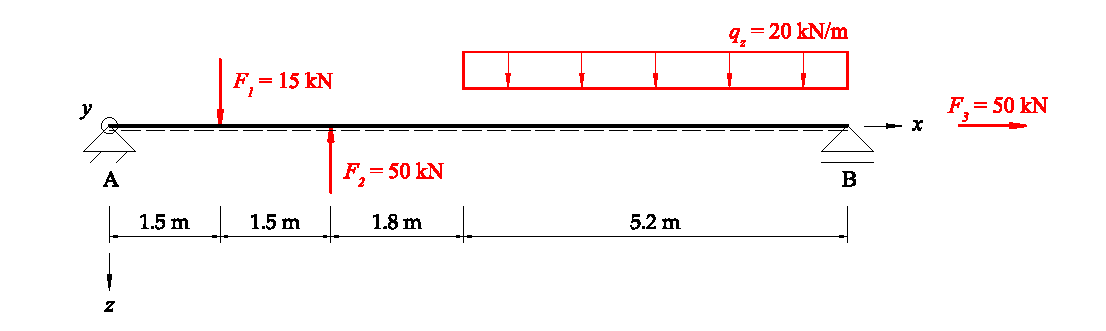
\includegraphics{BSI_HS23_Testat_01_files/mediabag/../images/Testat_01_HS23.pdf}

}

\caption{\label{fig-system}Ein einfacher Balken mit Streckenlast und
Punktlasten}

\end{figure}

Gesucht:

\begin{itemize}
\tightlist
\item
  Zeichnen Sie ein Schnittkörperdiagramm des gesamten statischen Systems
  (SKD) und bestimmen Sie die Lagerkraftgrössen in \(A\) und \(B\).
\item
  Kontrollieren Sie Ihre Berechnung der Lagerkraftgrössen.
\item
  Bestimmen Sie die Schnittgrössen Normalkraft \(N_x\), Querkraft
  \(V_z\) und Biegemoment \(M_y\) an der Stelle \(x=4\) m.
\end{itemize}

\newpage{}

\hypertarget{testat-1---musterluxf6sung}{%
\section{Testat 1 - Musterlösung}\label{testat-1---musterluxf6sung}}

\hypertarget{schnittkuxf6rperdiagramm}{%
\subsection{Schnittkörperdiagramm}\label{schnittkuxf6rperdiagramm}}

Das Schnittkörperdiagramm für das gesamte System ist in
Abbildung~\ref{fig-skd} gezeigt. Es sind lediglich die Auflagersymbole
durch entsprechende Reaktionskräfte zu ersetzen.

\begin{figure}[H]

{\centering 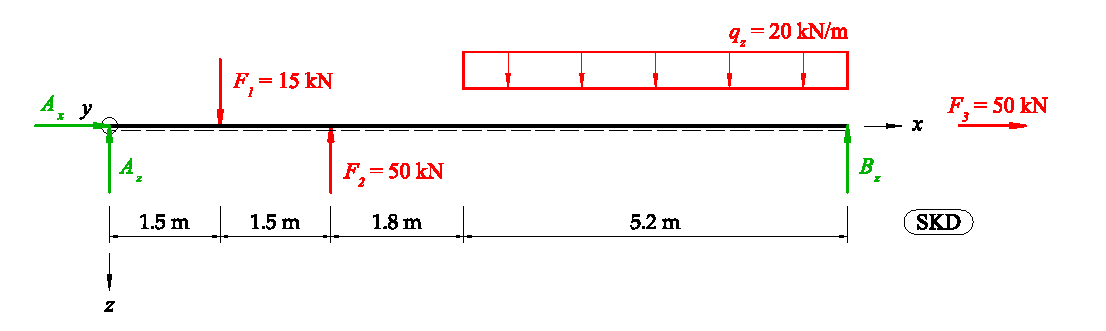
\includegraphics{BSI_HS23_Testat_01_files/mediabag/../images/Testat_01_HS23_SKD.pdf}

}

\caption{\label{fig-skd}Schnittkörperdiagramm des einfachen Balkens}

\end{figure}

\hypertarget{auflagerkruxe4fte}{%
\subsection{Auflagerkräfte}\label{auflagerkruxe4fte}}

Zuerst wird \(B_z\) ermittelt, dies kann durch Gleichgewicht der Momente
um Punkt \(A\) geschehen.

\begin{equation}\protect\hypertarget{eq-ggw_M_A}{}{
\sum_A^\curvearrowleft M_y = 0
}\label{eq-ggw_M_A}\end{equation}

\begin{equation}0 = B_{z} 10 \text{m} - F_{1} \cdot 1.5 \text{m} + F_{2} \cdot 3 \text{m} - q_{z} 5.2 \text{m} 7.4 \text{m}\end{equation}

\begin{equation}B_{z} = 3.848 q_{z} \text{m} + 0.15 F_{1} - 0.3 F_{2}\end{equation}

\begin{equation}B_{z} = 72154.0 \text{N}\end{equation}

Anhand des Momentengleichgewichts um Punkt \(B\) kann \(A_z\) ermittelt
werden. \begin{equation}\protect\hypertarget{eq-ggw_M_B}{}{
\sum_B^\curvearrowleft M_y = 0
}\label{eq-ggw_M_B}\end{equation}

\begin{equation}0 = - A_{z} 10 \text{m} + F_{1} \cdot 8.5 \text{m} - F_{2} \cdot 7 \text{m} + q_{z} 5.2 \text{m} 2.6 \text{m}\end{equation}

\begin{equation}A_{z} = 1.352 q_{z} \text{m} + 0.85 F_{1} - 0.7 F_{2}\end{equation}

\begin{equation}A_{z} = 446.0 \text{N}\end{equation}

Die horizontale Auflagerreaktion \(A_x\) kann durch Gleichgewicht der
horizontalen Kräfte ermittelt werden:

\begin{equation}\protect\hypertarget{eq-sum_fx}{}{
\sum^\rightarrow F_x = 0
}\label{eq-sum_fx}\end{equation}

\begin{equation}0 = A_{x} + F_{3}\end{equation}

\begin{equation}A_{x} = - F_{3}\end{equation}

\begin{equation}A_{x} = - 50000.0 \text{N}\end{equation}

\hypertarget{kontrolle-der-lagerkraftgruxf6ssen}{%
\subsection{Kontrolle der
Lagerkraftgrössen}\label{kontrolle-der-lagerkraftgruxf6ssen}}

Da beide Auflagerkräfte in \(z\)-Richtung mittels eines
Momentengleichgewichts bestimmt worden sind, bleibt die Summe aller
Kräfte in \(z\)-Richtung zur Kontrolle der Grössen.

\begin{equation}\protect\hypertarget{eq-ggw_fz}{}{
\sum^\uparrow F_z = 0
}\label{eq-ggw_fz}\end{equation}

\begin{equation}0 = 5.2 q_{z} \text{m} - A_{z} - B_{z} + F_{1} - F_{2}\end{equation}

\begin{equation}0 = 72600.0 \text{N} - A_{z} - B_{z}\end{equation}

\begin{equation}0 = 0\end{equation}

Es zeigt sich, dass die Gleichgewichtsbedingung auch in \(z\)-Richtung
eingehalten ist.

\hypertarget{schnittkruxe4fte}{%
\subsection{Schnittkräfte}\label{schnittkruxe4fte}}

Die Schnittkräfte lassen sich anhand eines SKDs bestimmen. Dabei ist das
System an der gewünschten Stelle zu schneiden. Am Schnittufer sind die
Schnittkräfte einzuführen. Dabei ist die Vorzeichenkonvention zu
beachten, welche sich anhand des Schnittufers (positv / negativ)
unterscheidet. Die Wahl des Schnittufers ist nicht relevant, da sich die
Schnittkräfte an diesem Punkt im Gleichgewicht befinden, sind die
Resultate identisch.

\begin{figure}[H]

{\centering 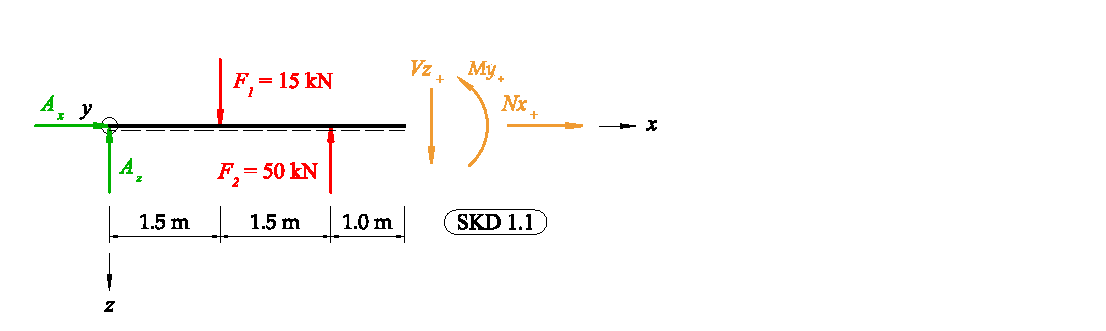
\includegraphics{BSI_HS23_Testat_01_files/mediabag/../images/Testat_01_HS23_SKD_1.pdf}

}

\caption{\label{fig-skd_4_pos}Schnittkörperdiagramm an der Stelle
\(x=4\)m mit positivem Schnittufer}

\end{figure}

\begin{figure}[H]

{\centering 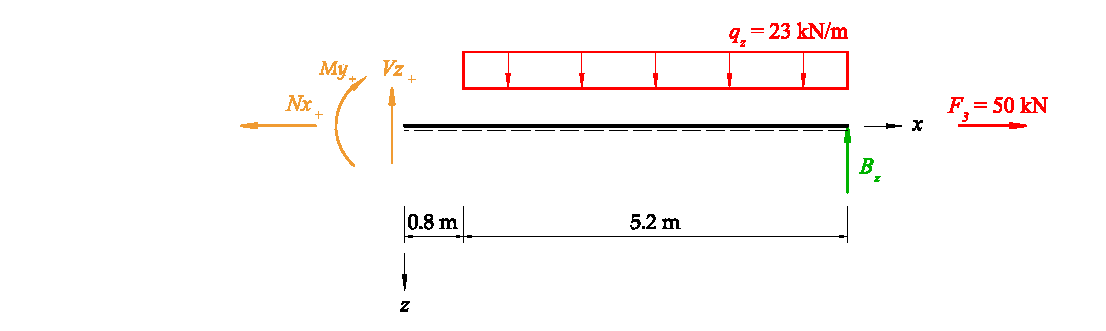
\includegraphics{BSI_HS23_Testat_01_files/mediabag/../images/Testat_01_HS23_SKD_2.pdf}

}

\caption{\label{fig-skd_4_neg}Schnittkörperdiagramm an der Stelle
\(x=4\)m mit negativem Schnittufer}

\end{figure}

Die Abbildung~\ref{fig-skd_4_pos} und Abbildung~\ref{fig-skd_4_neg}
zeigen ein negatives und positives Schnittufer für die gleiche Stelle im
System. Zur Ermittlung der Schnittkräfte gilt es nun die
Gleichgewichtsbedingungen anzuwenden.

Für das System in Abbildung~\ref{fig-skd_4_pos}, die Bestimmung der
Querkraft:

\begin{equation}\protect\hypertarget{eq-ggw_fz2}{}{
\sum_{x=4m}^\uparrow F_z = 0
}\label{eq-ggw_fz2}\end{equation}

\begin{equation}0 = A_{z} - F_{1} + F_{2} - V_{z}{\left(4 \text{m} \right)}\end{equation}

\begin{equation}V_{z}{\left(4 \text{m} \right)} = A_{z} - F_{1} + F_{2}\end{equation}

\begin{equation}V_{z}{\left(4 \text{m} \right)} = 47446.0 \text{N}\end{equation}

Die Bestimmung der Normalkraft:

\begin{equation}\protect\hypertarget{eq-sum_fx2}{}{
\sum_{x=4m}^\rightarrow F_x = 0
}\label{eq-sum_fx2}\end{equation}

\begin{equation}0 = A_{x} + N_{x}{\left(4 \text{m} \right)}\end{equation}

\begin{equation}N_{x}{\left(4 \text{m} \right)} = - A_{x}\end{equation}

\begin{equation}N_{x}{\left(4 \text{m} \right)} = 50000.0 \text{N}\end{equation}

Letztlich die Bestimmung des Biegemoments:

\begin{equation}\protect\hypertarget{eq-ggw_M_B_4m}{}{
\sum_{x=4m}^\curvearrowleft M_y = 0
}\label{eq-ggw_M_B_4m}\end{equation}

\begin{equation}0 = - A_{z} 4.0 \text{m} + F_{1} \cdot 2.5 \text{m} - F_{2} \cdot 1.0 \text{m} + M_{y}{\left(4 \text{m} \right)}\end{equation}

\begin{equation}M_{y}{\left(4 \text{m} \right)} = 0.5 \cdot \left(8.0 A_{z} - 5.0 F_{1} + 2.0 F_{2}\right) \text{m}\end{equation}

\begin{equation}M_{y}{\left(4 \text{m} \right)} = 26284.0 \text{m} \text{N}\end{equation}



\end{document}
